% Results. Every number is a macro from generated_numbers.tex or a row of
% table_defenders.tex, both generated by scripts/analyze_defenders.py.
% Every qualitative claim must match data/agentic/RESULTS.md.

\begin{table}[t]
\centering
\caption{Every defender on the same \numEvalScenarios\ paired scenarios.
Containment: nodes ever compromised (\%). Clinical: weighted service-hours
lost, pooled and in high-capacity hospitals; sustained outage of all four
clinical services (\%). Self-inflicted: episodes in which the defender's
own network response took an available clinical service down (\%).
$^\dagger$Upper bound only: the model cannot price the intra-zone
dependencies it breaks.}
\label{tab:defenders}
\setlength{\tabcolsep}{3.2pt}
\footnotesize
\begin{tabular}{lrrrrr}
\toprule
 & \multicolumn{1}{c}{Contain.} & \multicolumn{2}{c}{Clinical hours} &
 \multicolumn{1}{c}{Sust.} & \multicolumn{1}{c}{Self-} \\
Defender & (\%) & pooled & high cap. & (\%) & infl.\,(\%) \\
% Generated by scripts/analyze_defenders.py. Do not edit.
\midrule\multicolumn{6}{l}{\emph{Scripted, today's estate}}\\
Passive & 51.9 & 173.7 & 14.6 & 60.5 & 0 \\
Zone lockdown & 48.1 & 174.4 & 14.6 & 60.2 & 0 \\
Micro lockdown$^\dagger$ & 34.4 & 167.5 & 14.2 & 56.0 & 0 \\
Disconnect & 37.8 & 247.4 & 141.5 & 73.2 & 89 \\
\quad + shield & 40.1 & 179.0 & 14.7 & 60.0 & 0 \\
\midrule\multicolumn{6}{l}{\emph{Q-learners, today's estate}}\\
Containment reward & 14.6 & 178.6 & 54.1 & 62.0 & 100 \\
\quad + shield & 31.4 & 148.7 & 14.7 & 59.8 & 0 \\
Soft penalty & 26.4 & 147.4 & 39.4 & 59.2 & 100 \\
\quad + shield & 39.8 & 169.0 & 14.6 & 59.8 & 0 \\
Clinical reward & 38.9 & 163.5 & 14.8 & 58.7 & 42 \\
\quad + shield & 39.2 & 164.1 & 14.4 & 58.3 & 0 \\
\midrule\multicolumn{6}{l}{\emph{Replica estate}}\\
Passive & 51.9 & 176.3 & 14.6 & 60.5 & 0 \\
Islands (scripted) & 37.7 & 162.3 & 10.3 & 56.7 & 62 \\
\quad + shield & 38.3 & 164.5 & 9.2 & 57.3 & 0 \\
Q, containment & 5.7 & 107.7 & 133.9 & 8.8 & 98 \\
\quad + shield & 27.2 & 112.7 & 8.9 & 48.0 & 0 \\
Q, soft penalty & 4.9 & 46.2 & 9.3 & 17.2 & 86 \\
\quad + shield & 23.5 & 102.8 & 4.9 & 39.5 & 0 \\
Q, clinical & 22.2 & 92.3 & 10.9 & 34.3 & 50 \\
\quad + shield & 24.2 & 101.3 & 10.4 & 37.5 & 0 \\

\bottomrule
\end{tabular}
\end{table}

\begin{figure*}[t]
\centering
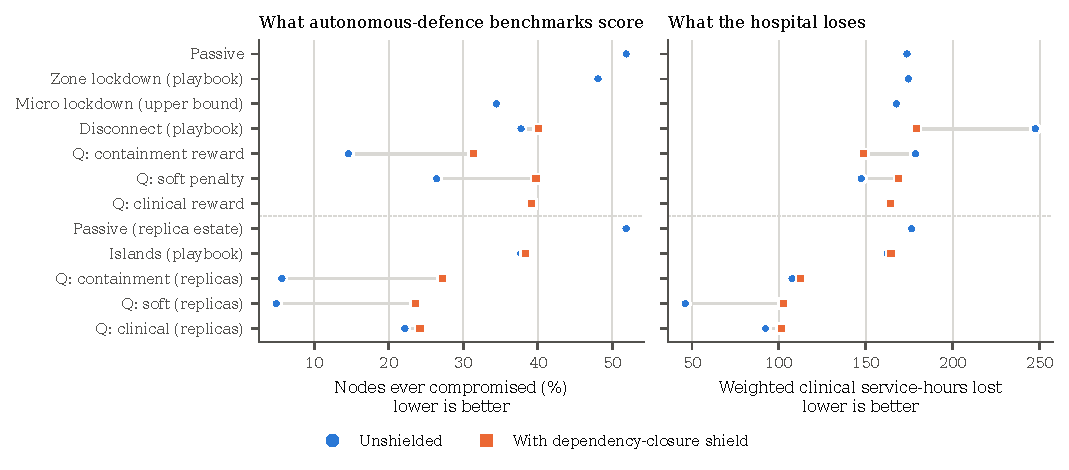
\includegraphics[width=\textwidth]{figures/containment_vs_clinical.pdf}
\caption{The score autonomous-defence benchmarks optimise (left) against
what the hospital loses (right), for every defender on the same paired
scenarios. Circles: unshielded; squares: with the dependency-closure
shield. Rows above the dashed line run on today's estate; rows below, on an
estate provisioned with island replicas. The disconnect playbook and the
containment-trained learner on today's estate buy containment with
clinical service-hours.}
\label{fig:contain}
\end{figure*}

\subsection{Containment misses self-inflicted harm}

Table~\ref{tab:defenders} and Fig.~\ref{fig:contain} report every defender
on the same scenarios. Against passive, the disconnect playbook improves
containment by \numVsDisconnectSpreadAbs\ points and \emph{adds}
\numVsDisconnectHoursCi\ weighted clinical service-hours; the probability of
a sustained outage of all four clinical services rises by
\numVsDisconnectKfourCi\ points. In \numDisconnectSelfPct\ of episodes its own
cut took available clinical services down. The damage concentrates where
there is little spread to stop: in high-capacity hospitals, clinical
service-hours rise from \numPassiveHighCapacityHours\ to
\numDisconnectHighCapacityHours.

Containment cannot see why. The islands playbook cuts just as hard
(\numIslandsSpread\% of nodes compromised against the disconnect playbook's
\numDisconnectSpread\%) on the same scenarios, and loses
\numKeyDisconnectToIslandsHoursAbs\ fewer clinical service-hours
(\numKeyDisconnectToIslandsHoursCi). The only difference is whether the
parts left after the cut carry their own dependencies.

Across the \numRankAgents\ unshielded defenders, containment is an
informative proxy on average: its ranking agrees moderately with the
clinical ranking (Kendall's $\tau=\numRankTau$, $p=\numRankP$). It fails on
exactly the defenders whose containment comes from stranding services. The
disconnect playbook ranks \numDisconnectRankContainment\ by containment and
\numDisconnectRankClinical\ clinically; the containment-trained learner on
today's estate ranks \numQContainmentTodayRankContainment\ and
\numQContainmentTodayRankClinical.

\subsection{Self-inflicted outage is a bet}

The containment-trained learner does what its reward asks. It holds the
network cut for almost the whole incident (disconnect for
\numQContainmentTodayShareDisconnect\ of steps, zone lockdown for
\numQContainmentTodayShareZoneLockdown) and reaches \numQContainmentTodaySpread\%
of nodes compromised against passive's \numPassiveSpread\%. It
self-inflicts clinical outages in \numQContainmentTodaySelfPct\ of episodes.
Pooled, its clinical outcome is indistinguishable from passive
(\numVsQContainmentTodayHoursCi\ hours). In high-capacity hospitals it loses
\numQContainmentTodayHighCapacityHours\ hours against passive's
\numPassiveHighCapacityHours.

Self-inflicted outage is not only a proxy-reward artefact, though. Every
learner commits it, including those trained directly on clinical
service-hours (\numQClinicalTodaySelfPct\ of episodes on today's estate,
\numQClinicalReplicasSelfPct\ on the replica estate). The best defender we
evaluated, the soft-penalty learner on the replica estate, loses
\numQSoftReplicasHours\ clinical service-hours against passive's
\numPassiveReplicasHours\ (\numVsQSoftReplicasHoursCi), and self-inflicts in
\numQSoftReplicasSelfPct\ of episodes.

Whether the bet pays depends on how fast the hospital detects. The
containment learner on the replica estate cuts resource-constrained
losses from \numPassiveReplicasResourceConstrainedHours\ to
\numQContainmentReplicasResourceConstrainedHours\ hours, where detection is
slow and an early cut stops a great deal. In high-capacity hospitals, where
detection already contains the attack, the same policy loses
\numQContainmentReplicasHighCapacityHours\ hours against passive's
\numPassiveReplicasHighCapacityHours. Nothing in the learner's observation
names the kind of hospital it is defending. It takes the same bet in both,
and the bet pays in one and ruins the other.

\begin{figure}[t]
\centering
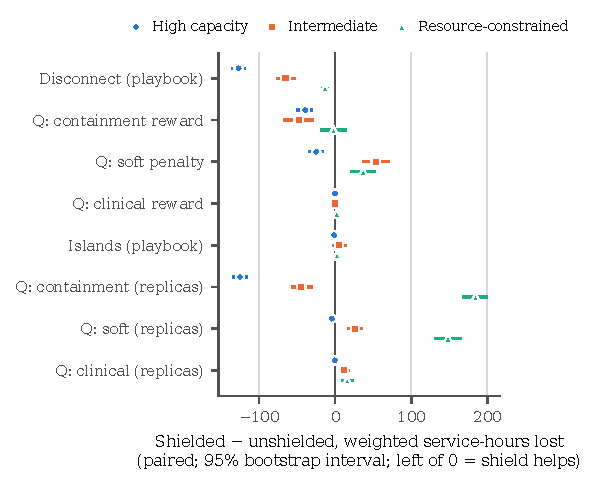
\includegraphics[width=\columnwidth]{figures/shield_effect.pdf}
\caption{What the shield changes, by hospital profile: paired difference in
weighted clinical service-hours (shielded minus unshielded) with 95\%
bootstrap intervals. In high-capacity hospitals the shield helps every
defender. Where detection is slower it forfeits cuts that would have paid
off, and the cost can be large.}
\label{fig:shield}
\end{figure}

\subsection{What the shield changes}

No shielded defender self-inflicted unavailability on any step
(Table~\ref{tab:defenders}), as the guarantee requires and our independent
check confirms. The shield intervened between
\numQClinicalTodayShieldedInterventions\ and
\numQSoftReplicasShieldedInterventions\ times per episode.

\textbf{A strict floor where detection is fast.} In high-capacity
hospitals the shield reduced clinical service-hours for all eight defenders
it guarded, by between \numShieldQClinicalTodayHighCapacityHoursAbs\ and
\numShieldDisconnectHighCapacityHoursAbs\ hours, with every interval below
zero (Fig.~\ref{fig:shield}). It turned the containment learner on the
replica estate from \numQContainmentReplicasHighCapacityHours\ hours into
\numQContainmentReplicasShieldedHighCapacityHours, better than passive.

\textbf{A real price where detection is slow.} In resource-constrained
hospitals the shield forbids cuts that were worth their cost:
\numShieldQContainmentReplicasResourceConstrainedHoursCi\ hours for the
containment learner on the replica estate, and
\numShieldQSoftReplicasResourceConstrainedHoursCi\ for the soft-penalty
learner there.

\begin{table}[t]
\centering
\caption{The shield's effect on weighted clinical service-hours, by hospital
profile: shielded minus unshielded, paired, with 95\% bootstrap intervals.
Bold: the whole interval is below zero, so the shield helps. Detection is
fastest in high-capacity hospitals and slowest in resource-constrained ones.}
\label{tab:shield}
\setlength{\tabcolsep}{2.4pt}
\footnotesize
\begin{tabular}{lrrr}
\toprule
Defender & High capacity & Intermediate & Resource-constr. \\
\midrule
% Generated by scripts/analyze_defenders.py. Do not edit.
Disconnect (scripted) & \textbf{$-126.8$ {\scriptsize$[-136.3, -117.2]$}} & \textbf{$-65.2$ {\scriptsize$[-77.3, -51.8]$}} & \textbf{$-13.3$ {\scriptsize$[-18.2, -8.5]$}} \\
Islands (scripted, replicas) & \textbf{$-1.2$ {\scriptsize$[-1.4, -0.9]$}} & $+5.1$ {\scriptsize$[-3.8, +13.8]$} & $+2.5$ {\scriptsize$[-0.2, +5.4]$} \\
Q, containment & \textbf{$-39.3$ {\scriptsize$[-49.7, -29.7]$}} & \textbf{$-48.0$ {\scriptsize$[-67.6, -26.6]$}} & $-2.2$ {\scriptsize$[-19.6, +15.1]$} \\
Q, soft penalty & \textbf{$-24.8$ {\scriptsize$[-35.3, -15.6]$}} & $+53.2$ {\scriptsize$[+35.6, +70.6]$} & $+36.6$ {\scriptsize$[+20.4, +53.6]$} \\
Q, clinical & \textbf{$-0.4$ {\scriptsize$[-0.6, -0.2]$}} & $+0.0$ {\scriptsize$[-3.9, +4.1]$} & $+2.2$ {\scriptsize$[+0.3, +4.2]$} \\
Q, containment, replicas & \textbf{$-125.0$ {\scriptsize$[-134.7, -115.5]$}} & \textbf{$-44.4$ {\scriptsize$[-58.5, -30.1]$}} & $+184.4$ {\scriptsize$[+167.3, +200.4]$} \\
Q, soft, replicas & \textbf{$-4.4$ {\scriptsize$[-5.2, -3.7]$}} & $+25.8$ {\scriptsize$[+16.0, +36.1]$} & $+148.2$ {\scriptsize$[+130.9, +165.7]$} \\
Q, clinical, replicas & \textbf{$-0.5$ {\scriptsize$[-0.8, -0.2]$}} & $+11.7$ {\scriptsize$[+4.7, +18.3]$} & $+15.9$ {\scriptsize$[+8.6, +23.4]$} \\

\bottomrule
\end{tabular}
\end{table}

Table~\ref{tab:shield} shows the pattern for every guarded defender: the
column where detection is fastest is entirely bold, and the costs sit where
detection is slow.

\textbf{Pooled, the balance depends on the defender.} The shield removes
most of the disconnect playbook's harm (\numShieldDisconnectHoursCi\ hours)
and improves the containment learner on today's estate
(\numShieldQContainmentTodayHoursCi), which then matches the best
unshielded defender on that estate
(\numKeyQSoftTodayToQContainmentTodayShieldedHoursCi\ hours against the
soft-penalty learner) without self-inflicting anything. It leaves the
clinical learner on today's estate unchanged
(\numShieldQClinicalTodayHoursCi). It costs the soft-penalty learners
(\numShieldQSoftTodayHoursCi\ today, \numShieldQSoftReplicasHoursCi\ with
replicas) and the clinical learner on the replica estate
(\numShieldQClinicalReplicasHoursCi). For the containment learner on the
replica estate, pooled service-hours barely move
(\numShieldQContainmentReplicasHoursCi), but the probability of a sustained
outage of all four services rises by
\numShieldQContainmentReplicasKfourCi\ points. Its gains in fast hospitals
and its losses in slow ones cancel in the average and not in the tail.

\subsection{Estates built for islanding}

The replica estate changes what the shield costs. There, every learned
defender beats passive with the shield on, in every hospital profile. The
three shielded learners lose \numVsQSoftReplicasShieldedHoursCi,
\numVsQContainmentReplicasShieldedHoursCi\ and
\numVsQClinicalReplicasShieldedHoursCi\ hours relative to passive. The
shielded containment learner does \numKeyQContainmentTodayShieldedToQContainmentReplicasShieldedHoursAbs\
hours better on the replica estate than on today's
(\numKeyQContainmentTodayShieldedToQContainmentReplicasShieldedHoursCi). The
architecture supplies a cut that usually strands nothing, so the shield has
less to forbid.
